% Сборка: latexmk -pdf -output-directory=build journal.tex && cp build/journal.pdf .
%
% Исследовательский журнал трека, черновик статьи: ландшафт подробно,
% эксперимент одним главным пунктом. Библиография --- refs.bib, новая запись
% только после сверки с первоисточником (arXiv ID или DOI).
\documentclass[11pt]{article}
\usepackage[T2A]{fontenc}
\usepackage[utf8]{inputenc}
\usepackage[russian]{babel}
\usepackage{amsmath,amssymb}
\usepackage[a4paper,left=2.2cm,right=6.4cm,top=2.3cm,bottom=2.3cm,
            marginparwidth=4.6cm,marginparsep=0.6cm]{geometry}
\usepackage{xcolor}
\usepackage{enumitem}
\usepackage{graphicx}
\usepackage{booktabs}
\usepackage{array}
\usepackage{framed}
\usepackage[numbers,sort&compress]{natbib}
\usepackage[hidelinks]{hyperref}

\definecolor{accent}{HTML}{9B1B1B}
\newcommand{\note}[1]{\marginpar{\raggedright\footnotesize\color{accent}#1}}
\newcommand{\Lfin}{L_{\mathrm{fin}}}
\graphicspath{{figures/}}

\title{\textbf{Эпиплексия синтетических данных\\
и качество моделей временных рядов}}
\author{Исследовательский журнал, черновик статьи}
\date{начат 23 октября 2026}

\begin{document}
\maketitle

\section{Введение}

Фундаментальная модель рядов прогнозирует ряды любой природы без
дообучения~\citep{ansari2025chronos2}. Помимо реальных рядов, такие модели
учат на синтетике: генератор задаёт распределение на случайных процессах,
приор, и модель, обученная на рядах из него, приближает байесовский
прогноз для этого приора~\citep{muller2022}. Какой генератор выбрать,
неизвестно. Одиннадцать генераторов при равном бюджете обучения дают
модели, различающиеся по качеству до двух раз, порядок генераторов зависит
от архитектуры, и способа выбрать генератор заранее нет~\citep{nagpal2026}.

Эпиплексия~\citep{finzi2026} есть количество выучиваемой структуры,
которую модель с ограниченным бюджетом вычислений извлекает из данных, на
практике площадь под кривой лосса над финальным лоссом. Гипотеза авторов:
перенос на новые задачи определяется эпиплексией данных, а не их лоссом.
Для языковых моделей она подтверждена на пяти доменах~\citep{su2026}.
Вопрос работы: от чего зависит качество модели, обученной на синтетике,
на реальных рядах, объясняет ли его эпиплексия генератора, и какой
функционал от генератора и модели обосновывает выбор генератора. Если
такой функционал есть, генераторы можно сравнивать без оценки на
бенчмарке.

\paragraph{Бенчмарк и метрики.} Бенчмарк есть набор реальных рядов из
разных областей: энергетика, транспорт, продажи, веб-трафик, медицина.
Каждый ряд разрезан на историю и будущее, модель видит только историю и
прогнозирует будущее на заданный горизонт. GIFT-Eval содержит такие задачи
для десятков наборов данных и частот, мы берём 55 задач с короткими
горизонтами, от 6 до 60 точек. Прогноз вероятностный: модель выдаёт
распределение будущих значений, на практике сотню траекторий. CRPS
измеряет расстояние между этим распределением и истинным значением, для
точечного прогноза он переходит в абсолютную ошибку, меньше лучше. MASE
измеряет абсолютную ошибку медианы прогноза. Обе метрики делятся на ошибку
сезонного наивного прогноза, который повторяет последний сезон, поэтому
значение меньше единицы значит лучше наива. Сводка по задачам:
геометрическое среднее отношений или средний ранг модели среди
сравниваемых. Связь предсказателя с качеством по одиннадцати генераторам
меряется корреляцией Спирмена, то есть согласием порядков, с
доверительным интервалом бутстрепом по генераторам.

\section{Ландшафт}

\subsection{Модели рядов и синтетика}

Модели табл.~\ref{tab:models} обучены на корпусах реальных рядов с добавкой
синтетики, три из них только на синтетике. Качество сравнивают на
GIFT-Eval~\citep{aksu2024} и fev-bench~\citep{shchur2025}, более ранний
архив Monash~\citep{godahewa2021} рассчитан на глобальные модели.

\begin{table}[t]
\centering
\small
\caption{Модели, их синтетика и качество на бенчмарках. Skill score, \%:
$1-{}$геометрическое среднее отношения CRPS (fev-bench: SQL) к сезонному
наиву по опубликованным результатам.}
\label{tab:models}
\footnotesize
\setlength{\tabcolsep}{4pt}
\makebox[\linewidth][l]{%
\begin{tabular}{@{}llrllrr@{}}
\toprule
Модель & Год & Размер & Архитектура & Синтетика & GIFT-Eval & fev-bench \\
\midrule
Chronos-Bolt                        & 2024 & 205M & T5, энкодер-декодер            & KernelSynth      & 42,6 & 38,9 \\
Sundial~\citep{liu2025sundial}      & 2025 & 128M & декодер, flow matching         & да               & 44,1 & 33,9 \\
TabPFN-TS~\citep{hoo2025}           & 2025 &      & табличный PFN                  & только синтетика & 45,6 &      \\
TempoPFN~\citep{moroshan2025}       & 2025 & 40M  & линейная RNN                   & только синтетика & 46,7 &      \\
Moirai-2.0~\citep{liu2025moirai2}   & 2025 & 11M  & декодер                        & KernelSynth      & 48,4 & 40,2 \\
Chronos-2-Synth~\citep{ansari2025chronos2} & 2025 & 120M & как Chronos-2           & только синтетика & 50,4 & 45,9 \\
TiRex~\citep{auer2025}              & 2025 & 35M  & xLSTM                          & да               & 51,2 & 42,7 \\
Chronos-2~\citep{ansari2025chronos2} & 2025 & 120M & энкодер, внимание между рядами & да              & 51,5 & 47,3 \\
Toto-2.0~\citep{khwaja2026}         & 2026 & 313M & декодер, внимание между рядами & да               & 51,9 & 44,2 \\
TiRex-2~\citep{podest2026}          & 2026 & 95M  & xLSTM, внимание между рядами   & сцепка рядов     & 52,2 & 45,5 \\
TimesFM-3.0                         & 2026 & 331M & декодер, внимание между рядами & да               & 54,4 & 48,7 \\
\bottomrule
\end{tabular}}
\end{table}

Синтетика для рядов делится на четыре вида: параметрические семейства
(ARIMA, ETS, GARCH), композиции базовых сигналов (тренд, сезонность,
ступеньки, волны), случайные процессы (гауссовские процессы, СДУ, fBm) и
нелинейные системы (хаотические аттракторы, NARMA).
KernelSynth~\citep{ansari2024}: гауссовский процесс с ядром из случайной
композиции базовых ядер. В абляции Chronos лучшая доля синтетики около
десятой части корпуса, а обучение только на синтетике хуже, чем с реальными
данными. TempoPFN~\citep{moroshan2025} обучен только на десяти генераторах,
в его абляции сильнее всего вредит удаление процессов Орнштейна--Уленбека с
переключением режимов (рис.~\ref{fig:tempo}). Многомерные способности
Chronos-2~\citep{ansari2025chronos2} получены из синтетики: одномерным
рядам навязывается многомерная структура.

\begin{figure}[t]
\centering
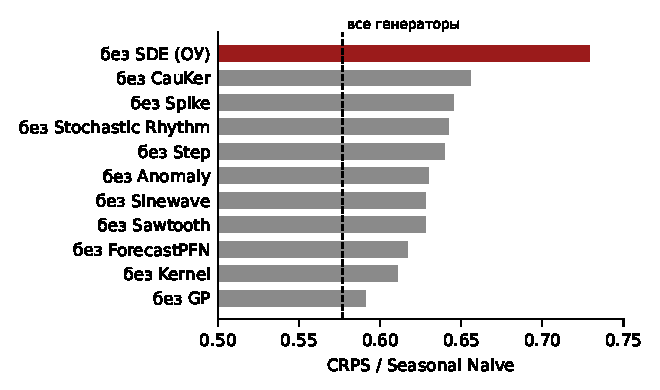
\includegraphics[width=0.6\linewidth]{tempopfn_loo.pdf}
\caption{TempoPFN: CRPS к наиву модели, обученной без одного генератора.}
\label{fig:tempo}
\end{figure}

Mix, Don't Pick~\citep{nagpal2026}: одиннадцать семейств генераторов
(KernelSynth, ETS, Waveform, SDE, StepFunction, TSI, ARIMA, fBm, GARCH,
Chaotic, TimeSynth), две архитектуры с нуля при равном бюджете, оценка без
дообучения на GIFT-Eval. Лучший и худший генератор различаются по CRPS в
полтора--два раза, порядок зависит от архитектуры (ETS второй у
Moirai-Small и худший у Chronos-T5-Mini), смесь всех генераторов с равными
весами не хуже лучшего, смесь реальных данных с синтетикой лучше обоих
чистых корпусов. Правила выбора генератора у авторов нет.

\subsection{Модель как байесовский предиктор}

Приор задаёт распределение $p(\theta)$ на процессах, процесс $\theta$
порождает ряд, окно ряда делится на контекст $c$ и будущее $f$.
Байесовский прогноз приора
\[
p(f\mid c)=\int p(f\mid c,\theta)\,p(\theta\mid c)\,d\theta
\]
есть лучший прогноз для рядов этого приора: его ожидаемый лог-лосс равен
условной энтропии $H(f\mid c)$, и ни один прогноз не даёт меньше. Модель
$q_\phi(f\mid c)$, обученная на окнах из приора с лог-лоссом, минимизирует
\[
\mathbb{E}_{c}\,\mathrm{KL}\bigl(p(\cdot\mid c)\,\|\,q_\phi(\cdot\mid c)\bigr)+H(f\mid c),
\]
то есть при достаточной ёмкости и данных сходится к байесовскому
прогнозу~\citep{muller2022}. Байесовский вывод оплачивается один раз при
обучении, на инференсе остаётся прямой проход. Два следствия для
синтетики. Модель, обученная на генераторе, есть приближение байесовского
прогноза этого генератора, и её качество на реальных рядах складывается из
того, насколько байесовский прогноз генератора хорош для реальных рядов, и
из ошибки приближения. Лосс обучения ограничен снизу энтропией
$H(f\mid c)$, и у генераторов с почти детерминированными рядами в
непрерывной плотности эта граница лежит сколь угодно низко, поэтому
сравнивать генераторы можно только при общей для всех точности или
отсчитывая лосс от известной границы.

Ошибка обучаемого предиктора раскладывается на три
части~\citep{jeon2024}. Для корпуса $H_{M,T}$ из $M$ задач длины $T$,
порождённых приором с параметром $\psi$, где $\theta_m$ параметр $m$-й
задачи, а $D_m$ её данные,
\[
\mathcal{L}_{M,T}
=\underbrace{\frac{\mathrm{H}(H_{M,T}\mid\theta_{1:M})}{MT}}_{\text{неустранимая}}
+\underbrace{\frac{\mathrm{I}(H_{M,T};\psi)}{MT}}_{\text{мета-обучение}}
+\underbrace{\frac{\mathrm{I}(D_m;\theta_m\mid\psi)}{T}}_{\text{внутри задачи}}.
\]
Первая часть есть шум процесса, третья цена вывести параметры ряда по
контексту при известном приоре, вторая цена выучить сам приор по корпусу,
равная взаимной информации между приором и корпусом. Это ошибка идеального
байесовского ученика, который видит корпус впервые. Накопленная по $N$
окнам, она есть нижняя граница площади над точной границей для любой
модели:
\[
A_{H}=\sum_{i=1}^{N}\ell_i-N\,H(f\mid c)\;\ge\;
A_{\mathrm{B}}=\sum_{i=1}^{N}\bigl(\mathbb{E}\,\ell^{\mathrm{B}}_i-H(f\mid c)\bigr),
\]
где $\ell_i$ лосс модели на $i$-м окне до шага по нему, а
$\ell^{\mathrm{B}}_i$ лосс байесовского ученика после $i-1$ предыдущих
окон. Для приора с $p$ непрерывными параметрами асимптотика
Кларка--Бэррона~\citep{clarke1990} даёт $A_{\mathrm{B}}=\tfrac{p}{2}\log
N+O(1)$: байесовская часть площади растёт логарифмически, а всё, что модель
набирает сверх неё, есть цена выучить сам алгоритм прогноза и точность
процесса.

У приоров с известным байесовским прогнозом граница и байесовский ученик
считаются точно. У процесса Орнштейна--Уленбека и у гауссовских процессов
с известным ядром апостериорный прогноз гауссов и выписывается в замкнутом
виде, у гауссовских семейств с конечным числом параметров $A_{\mathrm{B}}$
считается Монте-Карло. На таких оракульных генераторах площадь сети
раскладывается на обязательную байесовскую часть и избыток, который вносит
сама сеть.

\subsection{Эпиплексия}

\paragraph{Определение.} Среди программ, которые считают вероятность и
сэмплируют за время не больше $T$, берётся кратчайший двухчастный
код~\citep{finzi2026}:
\[
\mathrm{P}^\star=\arg\min_{\mathrm{P}\in\mathcal{P}_T}\Bigl(|\mathrm{P}|+\mathbb{E}\log\tfrac{1}{P(X)}\Bigr),
\qquad S_T(X)=|\mathrm{P}^\star|,\qquad H_T(X)=\mathbb{E}\log\tfrac{1}{P^\star(X)}.
\]
Эпиплексия $S_T$ есть длина лучшей модели при бюджете $T$, структурная
часть информации. Ограниченная по времени энтропия $H_T$ есть остаточный
лосс этой модели, случайная часть. У равномерного шума $S_T$ ограничена
константой, у периодического узора обе части $O(1)$, у криптографического
генератора псевдослучайных чисел структуры нет при почти максимальной
энтропии. С ростом бюджета сумма $S_T+H_T$ не растёт, обычно $S_T$ растёт,
а $H_T$ падает. Класс программ можно сузить до моделей, достижимых данной
архитектурой и оптимизатором, и тогда эпиплексия зависит от модели.

\paragraph{Оценка по кривой обучения.} На шаге $i$ пример $Z_i$ кодируется
текущей моделью за $\log 1/P_i(Z_i)$ нат, затем модель на нём обучается.
Сумма есть код данных вместе с финальными весами, а при известных
финальных весах данные стоят $\sum_i\log 1/P_M(Z_i)$. Разность есть длина
модели:
\[
A=\sum_{i=1}^{N}\ell_i-N\,\Lfin,
\]
площадь под кривой лосса над финальным лоссом, prequential-код
Блие и Оливье~\citep{blier2018} за вычетом лосса финальной модели. Лосс
снимается до шага по примеру, каждый пример виден впервые, одна эпоха.
Оценка нестрогая, но годится для ранжирования наборов данных по готовой
кривой. Строгая версия, requential-код~\citep{qiu2026}, кодирует веса
через учителя и в несколько раз короче при обычно том же порядке
наборов. Способы оценки разобраны в разделе~\ref{sec:estimators}.

\paragraph{Перенос.} Гипотеза~\citet{finzi2026}: перенос на новые задачи
определяется тем, сколько переиспользуемой структуры модель забрала в
веса, а не лоссом внутри распределения, и два корпуса с равным лоссом
могут переноситься по-разному. Подтверждения в статье косвенные:
шахматные записи в порядке доска$\to$ходы дают большую эпиплексию и
выигрыш на оценке позиции, адаптивный выбор доменов ADO~\citep{jiang2025}
поднимает эпиплексию вместе с точностью. Оговорка авторов: эпиплексия
меряет количество структуры, а не её уместность для конкретной задачи. На
натуральных данных структура оказалась малой долей информации: у текста
её больше всего, у картинок меньше всего.

\paragraph{Прямая проверка на языке.} \citet{su2026} обучили по модели на
каждом из пяти крупнейших доменов Pile за одну эпоху, оценили эпиплексию
по кривой лосса и качество на семи задачах вне доменов. Пирсон между ними
$0{,}88$, Спирмен $0{,}90$, норма весов как контроль не предсказывает.
Мелкие домены исключены, потому что потребовали бы повторов. На этой связи
построены EpiSelect (веса доменов по приросту эпиплексии, предсказанному
законами масштабирования на лету) и EpiGen (генератор синтетики с наградой
за падение лосса ученика). Наша схема та же: одиннадцать генераторов вместо
пяти доменов, GIFT-Eval вместо задач языка, и данные генераторов
бесконечны.

\paragraph{Возражения.} \citet{li2026} строит два корпуса: в первом много
структуры, не нужной целевой задаче, во втором меньше, но нужной.
Показатель общей структуры ставит выше первый, точность на сдвинутой задаче
выше у второго в двух сидах из трёх. На клеточных автоматах качество
последующих задач немонотонно по сложности правила~\citep{zhang2024}, а
лучшая сложность синтетики зависит от целевого домена~\citep{lee2026}.
Общая структура данных и структура, полезная для цели, могут расходиться.
Площадь зависит от рецепта обучения: шага, разогрева, батча,
расписания~\citep{bornschein2022}.

\paragraph{Базы для выбора данных.} DataDecide~\citep{magnusson2025}:
ранжирование корпусов по моделям одного малого размера угадывает победителя
на большом размере примерно в 80\,\% пар, экстраполяция по законам
масштабирования не лучше. ADO~\citep{jiang2025} перевзвешивает домены во
время обучения по законам масштабирования, подогнанным к кривым лосса.

\section{Способы оценки эпиплексии}\label{sec:estimators}

Эпиплексия определена через минимум по программам, который не вычислим, и
каждая оценка есть выбор класса моделей, рецепта обучения и точки отсчёта.
Ниже способы оценки, что каждый меряет и какие вопросы оставляет. Раздел
абстрактный и служит началом теоретической работы.

\paragraph{Площадь над отложенным лоссом.} $A=\sum_i\ell_i-N\Lfin$, где
$\Lfin$ лосс финальных (усреднённых) весов на свежих окнах того же
генератора. Нужна одна эпоха. Ошибка $\Lfin$ входит с множителем $N$.
Площадь растёт вместе с тем, насколько низко лосс может уйти на почти
детерминированных рядах, и зависит от рецепта обучения. Точку отсчёта
можно брать иначе: лосс на хвосте обучения, лосс первого прохода, минимум
по чекпойнтам. Все они меряют одно и то же с разным смещением.

\paragraph{Площадь над точной границей.} На оракульных приорах
$A_H=\sum_i\ell_i-N\,H(f\mid c)=A+N(\Lfin-H)$. Она раскладывается на
байесовскую часть $A_{\mathrm{B}}$ порядка $\log N$ и избыток сети. На
генераторах, где ряды почти детерминированы, избыток содержит цену выучить
точность процесса, то есть узость плотности, и эта цена растёт с
разрешением. Гипотеза: эпиплексия как функция разрешения $S(\sigma)$, где
$\sigma$ общая для всех генераторов точность, при которой считается лосс,
и генераторы сравниваются при одном $\sigma$; кривая $S(\sigma)$ есть
спектр структуры по масштабам. Для генераторов без оракула границу можно
оценивать подгонкой кривой $L(n)=E+a\,n^{-\alpha}$, а точность подгонки
проверять там, где граница известна.

\paragraph{Requential-код с оракульным учителем.} В~\citet{qiu2026} ученик
учится на примерах, сэмплированных из учителя, скользящего среднего самого
ученика, и длина кода равна $\sum_i\mathrm{KL}(P^{\mathrm{t}}_i\,\|\,P^{\mathrm{s}}_i)$.
На приоре с известным байесовским прогнозом учителем может быть сам
прогноз $p(f\mid c)$: тогда код равен $\sum_i\mathbb{E}_c\,
\mathrm{KL}(p(\cdot\mid c)\,\|\,q_i(\cdot\mid c))$, в ожидании это $A_H$.
У гауссовских процессов и Орнштейна--Уленбека учитель гауссов, и для
гауссовского ученика KL считается в замкнутом виде, для ученика со смесью
Монте-Карло по сэмплам учителя. Вопросы: как код с оракульным учителем
соотносится с кодом со скользящим учителем на одних приорах, и какой из них
ранжирует приоры так же, как площадь.

\paragraph{Компьют-оптимальный код.} При каждом бюджете $T$ по сетке
размеров модели и объёмов данных берётся кратчайший двухчастный код, его
части есть оценки $S_T$ и $H_T$~\citep{finzi2026}. Нужна линейка моделей.
Вопрос: как $S_T$ генераторов меняется с $T$ и с какого $T$ порядок
генераторов устанавливается.

\paragraph{Рецепт и единицы.} По определению минимум берётся и по рецептам
обучения, так что зависимость площади от шага и расписания есть ошибка
оценки. Можно брать общий рецепт, можно подбирать под каждый генератор и
брать минимум; мерить нужно устойчивость порядка генераторов, а не
абсолютные площади. Площади сравнимы только внутри одной модели: у разных
моделей лосс считается на разных объектах.

\section{Альтернативы эпиплексии}\label{sec:alternatives}

Нужен функционал от генератора и модели, который предсказывает качество
модели, обученной на генераторе, на реальных рядах. Эпиплексия один из
кандидатов. Требования к функционалу: он зависит от модели, потому что
порядок генераторов у двух архитектур разный и мера только по данным его
не объяснит; он не растёт с точностью на детерминированных рядах; он не
требует бенчмарка, иначе теряется смысл; он дешевле полного прогона или
хотя бы не дороже.

\begin{description}[leftmargin=0pt,labelindent=0pt,style=nextline,itemsep=2pt]
\item[Финальный лосс и падение лосса.] $\Lfin$ и $L_{\mathrm{start}}-\Lfin$
  меряют шумность генератора и точность, а не структуру; в единицах лосса
  несравнимы между генераторами.
\item[Меры без обучения.] Сжимаемость gzip, спектральная энтропия,
  разнообразие признаков ряда. Не зависят от модели и не объяснят разный
  порядок у двух архитектур, но дёшевы и дают базу.
\item[Лосс чужой модели.] Лосс или CRPS сильной модели, обученной на
  реальных рядах, на рядах генератора: насколько генератор знаком модели
  реальных данных. Прокси близости к реальным рядам, считается без
  обучения.
\item[Расстояние распределений.] Расстояние между окнами генератора и
  реальными окнами в пространстве признаков или эмбеддингов обученной
  модели: MMD, классификатор двух выборок. Прямая мера совпадения доменов.
\item[Условная эпиплексия.] Площадь на реальных рядах при дообучении
  модели, предобученной на генераторе: чем меньше, тем больше нужной
  структуры дала синтетика. Учитывает и количество структуры, и её
  уместность, но требует реальных данных.
\item[Предиктивная $\mathcal{V}$-информация.] Прирост качества прогноза
  реальных рядов от доступа к контексту для класса моделей, обученных на
  генераторе; определяется через семейство предикторов, а не через код.
\item[Информация корпуса о приоре.] Член мета-обучения $\mathrm{I}(H;\psi)$,
  число различимых по окну процессов, информация Фишера окна о процессе.
  Считаются на оракульных приорах и не зависят от сети: мера структуры
  самого приора.
\item[Короткие прогоны и малые модели.] Качество ранних чекпойнтов или малых
  моделей на части бенчмарка~\citep{magnusson2025}. Требует бенчмарк, но
  дёшево. Сюда же скорость начального падения лосса: по нашим прогонам
  площадь по первым окнам коррелирует с CRPS положительно, быстрый старт
  даёт худшие модели.
\item[Вклад в смесь.] Изменение качества смеси при удалении генератора.
  Практическая цель составления корпуса и больше точек для корреляции.
\item[Эпиплексия при фиксированном разрешении.] $S(\sigma)$ из
  раздела~\ref{sec:estimators}: та же площадь, но при общей для всех
  генераторов точности.
\end{description}

\section{Эксперимент}

Moirai-Small обучена с нуля на каждом из одиннадцати генераторов Mix,
Don't Pick при равном бюджете в сорок миллионов окон, один сид; площадь
над финальным лоссом против качества на 55 задачах GIFT-Eval. По всем
одиннадцати генераторам связи нет: Спирмен $0{,}00$ $[-0{,}89;\,+0{,}61]$ с
CRPS к наиву. Без Chaotic и Waveform связь есть, $-0{,}82$ и по CRPS, и по
MASE, в пользу гипотезы; подмножество выбрано после результата
(рис.~\ref{fig:s2}, кривые обучения на рис.~\ref{fig:s2curves}). По
первым $0{,}4$ млн окон корреляция с CRPS к наиву положительная, $+0{,}61$
$[+0{,}10;\,+0{,}88]$, и проходит через ноль к двум миллионам
(рис.~\ref{fig:s2corr}).

\begin{figure}[p]
\centering
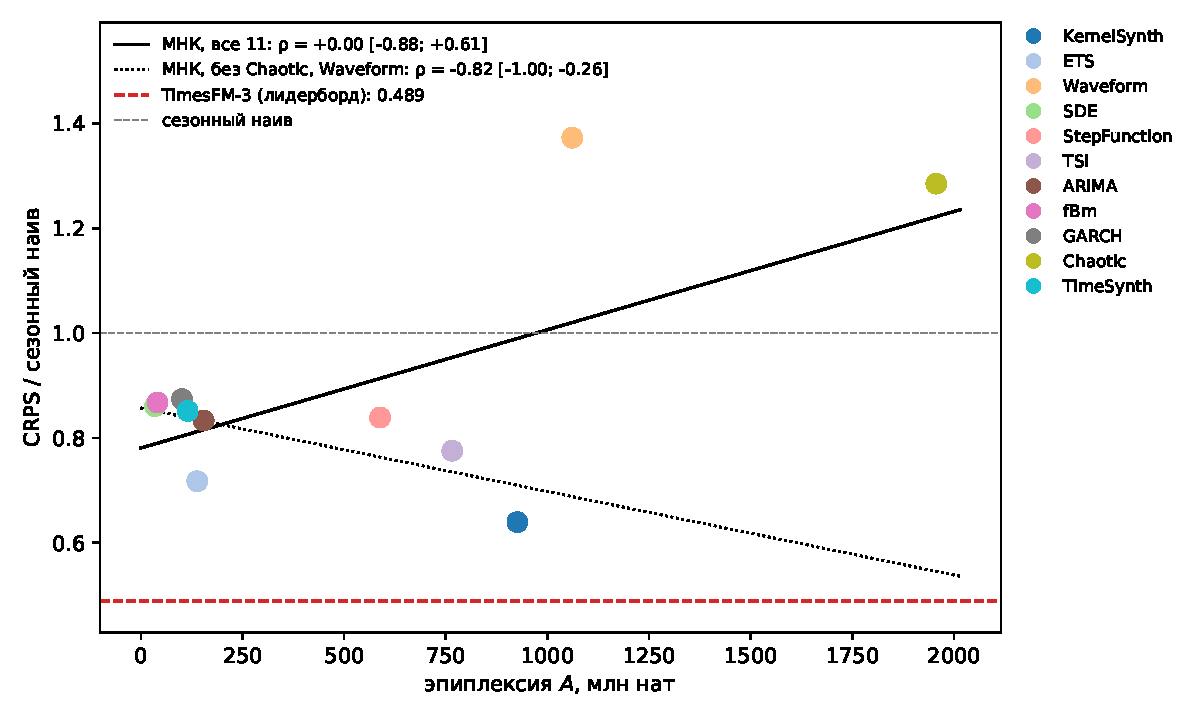
\includegraphics[width=0.82\linewidth]{s2_crps_vs_epiplexity_lines.pdf}\\[2pt]
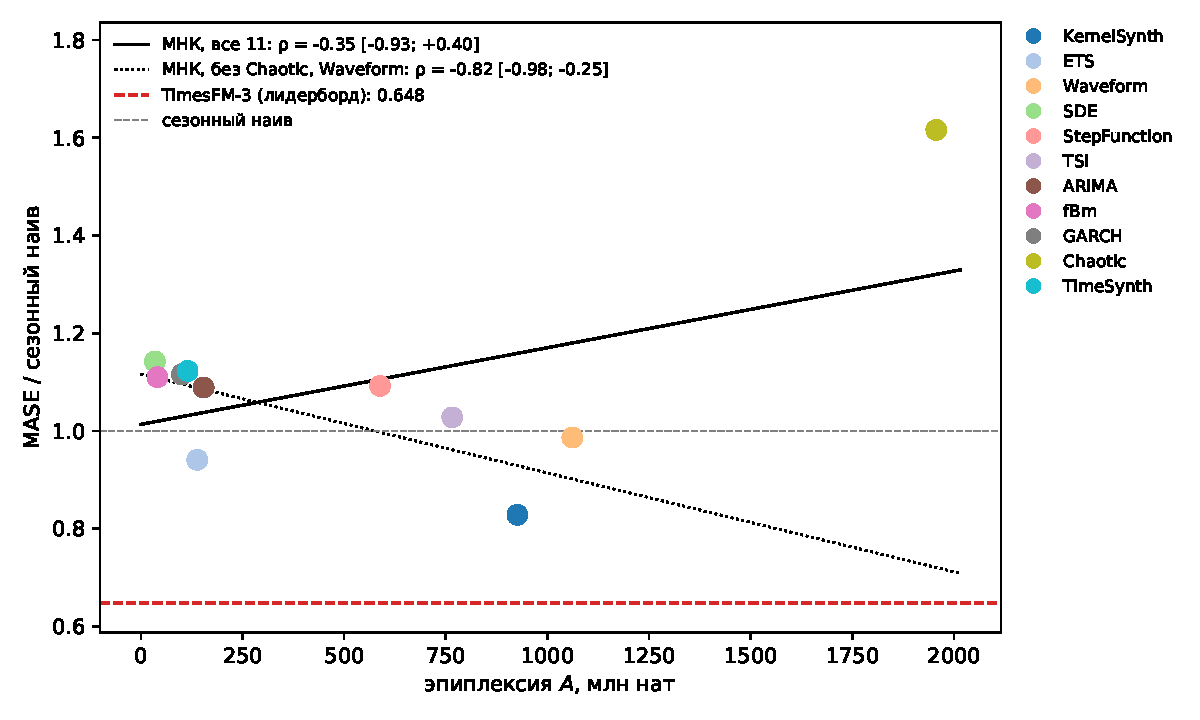
\includegraphics[width=0.82\linewidth]{s2_mase_vs_epiplexity_lines.pdf}
\caption{CRPS и MASE к сезонному наиву против площади. Прямые ---
регрессия по всем одиннадцати генераторам и по девяти без Chaotic и
Waveform, в легенде Спирмен с бутстреп-интервалом. Горизонталь ---
TimesFM-3 на тех же задачах.}
\label{fig:s2}
\end{figure}

\begin{figure}[p]
\centering
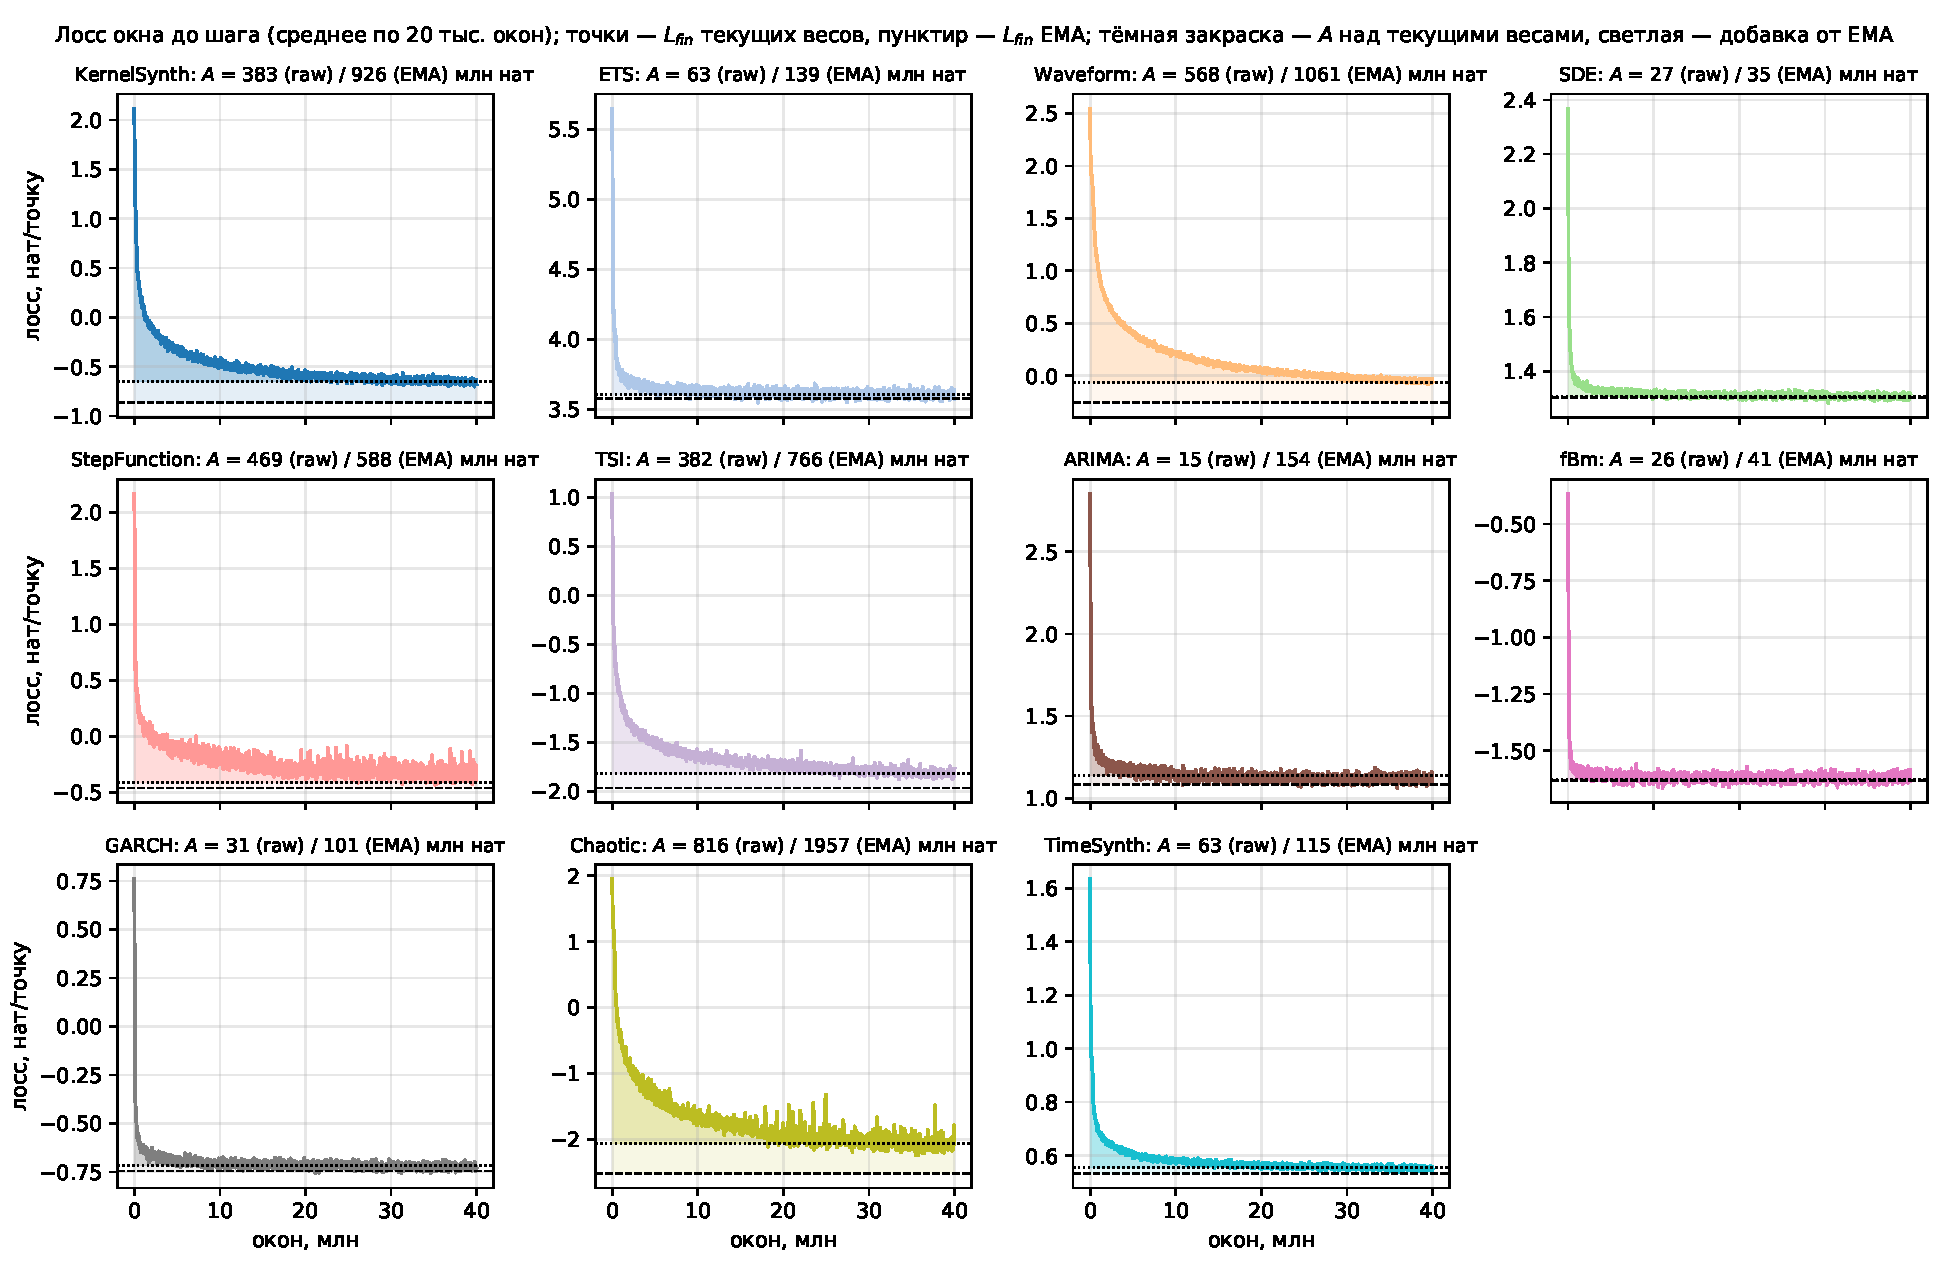
\includegraphics[width=\linewidth]{s2_train_curves_area.pdf}
\caption{Кривые обучения, лосс окна до шага. Точечная линия ---
$\Lfin$ текущих весов, пунктир --- усреднённых, закраска --- площадь.}
\label{fig:s2curves}
\end{figure}

\begin{figure}[p]
\centering
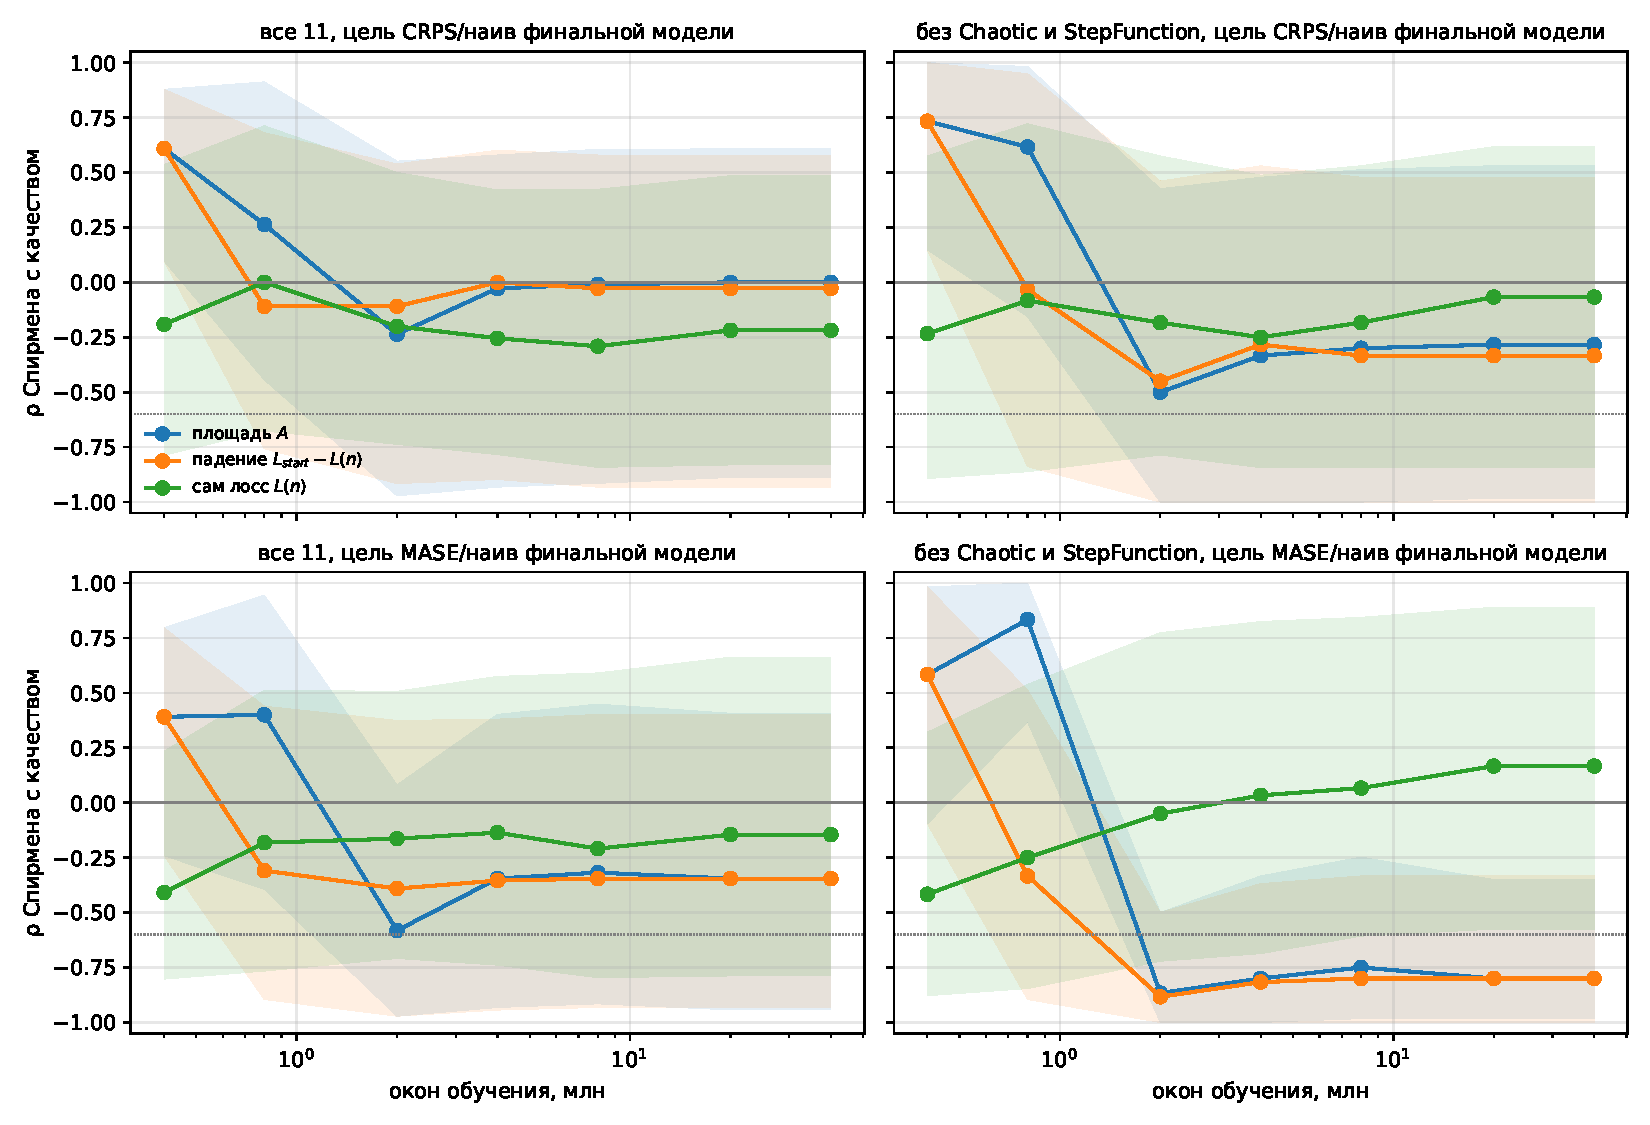
\includegraphics[width=\linewidth]{s2_corr_vs_windows.pdf}
\caption{Корреляция оценок по первым $n$ окнам с итоговым
качеством, полосы --- 95\,\% бутстреп по генераторам.}
\label{fig:s2corr}
\end{figure}

\clearpage
\section{Направления}

\paragraph{Эпиплексия для других лоссов.}\note{Пусть Лёша займётся
изучением.} Площадь равна длине кода только у лог-лосса. У любого строго
собственного правила оценки~\citep{gneiting2007} ожидаемый лосс
раскладывается на обобщённую энтропию и расхождение прогноза с истиной,
поэтому площадь над финальным лоссом есть накопленное расхождение, аналог
без связи с длиной описания. Лосс диффузии с весами ELBO задаёт
код~\citep{kingma2023}, с другими весами площадь нужно перевзвешивать, а
его нижнюю границу оценивает~\citet{xu2026}.

\begin{framed}
\noindent\textbf{Исследовательский вопрос.} Можно ли определить
эпиплексию для моделей, обученных не на лог-лоссе, так, чтобы площадь под
кривой обучения сохраняла смысл длины описания или хотя бы ранжировала
источники данных так же, как площадь лог-лосса.

\medskip\noindent\textbf{Постановка, варианты.}
\begin{enumerate}[nosep,leftmargin=1.4em]
\item Квантильный лосс. Сумма квантильных лоссов по сетке уровней
  приближает CRPS, а CRPS строго собственное правило, его расхождение есть
  интеграл квадрата разности функций распределения. Определить площадь как
  накопленное расхождение, выяснить, когда её порядок по источникам
  совпадает с порядком по KL, и оценить ошибку обходного пути: собрать из
  квантилей плотность и считать лог-лосс.
\item Диффузионный лосс. При весах ELBO площадь определена в натах. Выяснить,
  как площадь зависит от весов по уровням шума, какова её нижняя граница и
  как определить requential-код для диффузионной модели.
\item Общий случай. Для произвольного строго собственного правила площадь
  над финальным скором есть накопленная дивергенция Брегмана. Найти условия
  на семейство распределений, при которых ранжирование источников не
  зависит от правила.
\end{enumerate}

\medskip\noindent\textbf{Зачем для публикации.} Сильнейшие модели рядов
учатся на квантильном лоссе (Chronos-2, TiRex, Moirai 2.0) или на
диффузии и flow matching (Sundial), и эпиплексия в
определении~\citep{finzi2026} к ним неприменима. Расширение на другие
лоссы делает меру применимой к этим моделям и является теоретическим
результатом, не привязанным к рядам.
\end{framed}

\paragraph{Влияние генератора и рецепта.} Увеличивает ли эпиплексию
усложнение генератора и в каком смысле. Как площадь зависит от шага,
расписания, инициализации, и переживает ли порядок генераторов смену
рецепта.

\paragraph{Утолщённые многообразия.} Распределение на многообразии,
свёрнутое с гауссианой толщины $\sigma$: структура и шум заданы
конструкцией, истинная энтропия и байесовская кривая обучения известны.
Чистая проверка меры на непрерывных данных и источник кривой $S(\sigma)$.

\bibliographystyle{plainnat}
\bibliography{refs}

\end{document}
